\section{Results}
\label{sec:results}

The central finding is that the certified floor of Corollary~\ref{cor:floor} is
honoured empirically when the optimizer enforces the $\psi$-budget and is violated
when it does not. Table~\ref{tab:coverage} reports the two arms against the floor;
Figure~\ref{fig:coverage} shows the coverage decomposition and the per-cycle
mechanism.

\begin{table}[t]
\centering
\caption{Closed-loop coverage over $8$ seeds $\times\,80$ cycles ($N=640$ per arm).
The health-constrained arm meets the certified floor $0.75$; the health-blind arm
does not. Brackets are Wilson $95\%$ intervals.}
\label{tab:coverage}
\begin{tabular}{lccc}
\toprule
 & Health-blind & Health-constrained & Certified floor \\
 & ($\varepsilon\to\infty$) & ($\varepsilon=0.05$) & \\
\midrule
$S_k$ coverage & $0.000\,[0.000,0.006]$ & $\mathbf{0.988\,[0.976,0.994]}$ & $0.750$ \\
\quad meets floor? & no & \textbf{yes} & --- \\
Quality coverage $\{x_k\le x^{\mathrm{spec}}\}$ & $0.850$ & $0.988$ & --- \\
RUL coverage $\{\rho_k\ge\rho_{\min}\}$ & $0.013$ & $1.000$ & --- \\
$\psi$-budget binding & $0\%$ & $100\%$ & --- \\
Mean final severity & $0.700$ & $0.097$ & --- \\
\bottomrule
\end{tabular}
\end{table}

\begin{figure}[t]
\centering
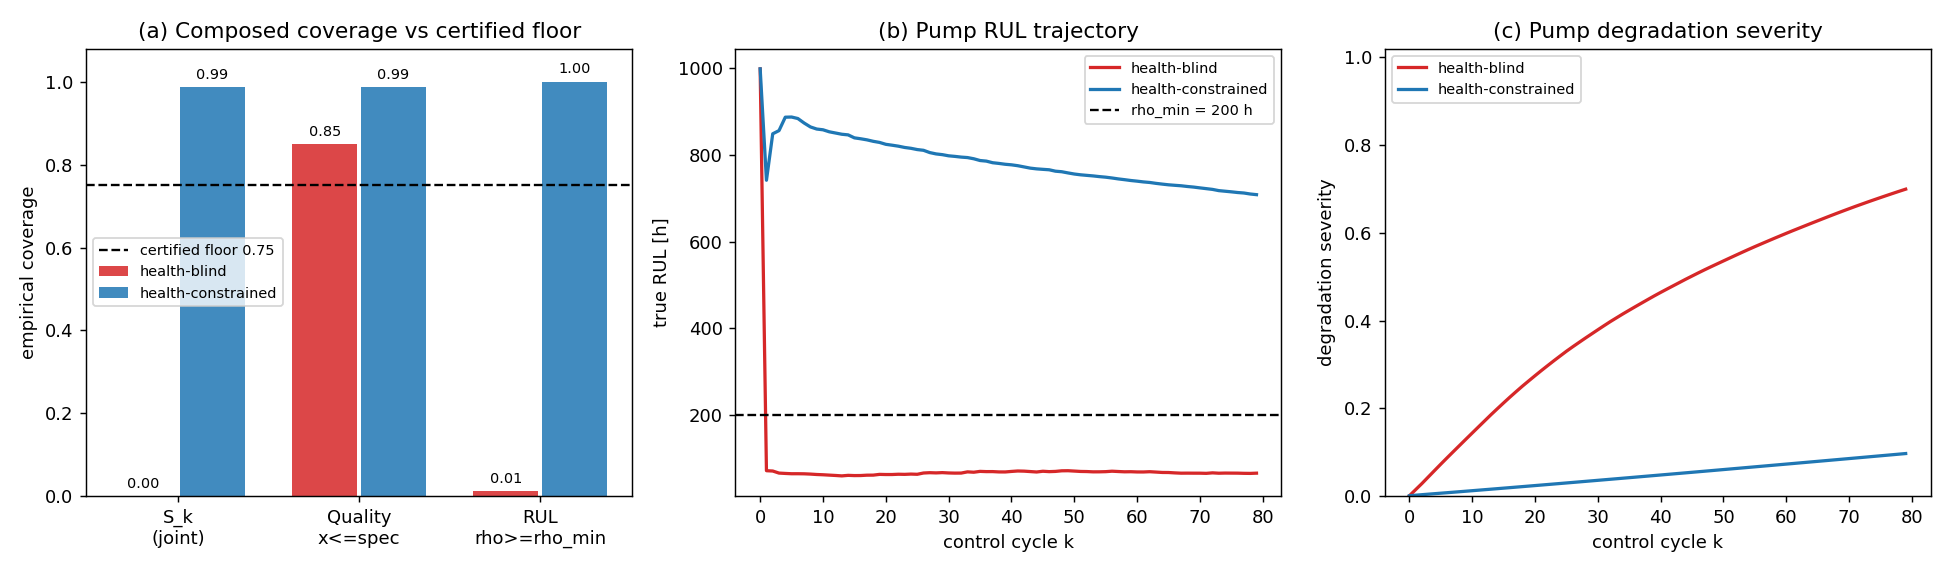
\includegraphics[width=\textwidth]{figures/twin_coverage.png}
\caption{Composed coverage certificate on the debutanizer twin.
(a) Empirical coverage of the joint safety event $S_k$ and its two halves for the
two arms, against the certified floor $1-(\alpha_1+\alpha_2)-\varepsilon=0.75$
(dashed). (b) True reflux-pump remaining life per cycle; the health-blind arm falls
below the floor $\rho_{\min}=200$~h within two cycles, the health-constrained arm
holds $700$--$1000$~h. (c) Degradation severity per cycle.}
\label{fig:coverage}
\end{figure}

\subsection{The certificate holds under the budget}
\label{sec:res-cert}

Under the $\psi$-budget the joint safety event holds on $0.988$ of cycles
($95\%$ Wilson interval $[0.976, 0.994]$), comfortably above the certified floor of
$0.75$. Both halves of $S_k$ are satisfied simultaneously: quality coverage is
$0.988$ and remaining-life coverage is $1.000$. The budget is active on every
constrained cycle, holding the operating point on the certified reference; the
reflux pump ends the horizon at a mean severity of $0.097$, far from its alarm.

The empirical coverage exceeds the floor by a wide margin. This is expected and
consistent with the construction: the certificate is a valid lower bound, and two
sources of conservatism inflate the gap --- the Bonferroni union over the two
miscoverage events (Theorem~\ref{thm:composed}), which is tight only when the two
failures are disjoint, and the deliberately conservative Lipschitz constants
($L_1=L_2=0.15$ against a swept $L_1\approx0.024$). The result to read from
Table~\ref{tab:coverage} is therefore the \emph{verdict} --- floor met with margin
--- not the size of the margin.

\subsection{The mechanism: why the blind optimizer fails}
\label{sec:res-mech}

The health-blind arm exposes what the budget protects against. Facing the same
tight specification, the unconstrained optimizer drives the reflux ratio to its
upper bound ($R\to3.0$, reflux flow $\approx\!97$~kmol\,h$^{-1}$) to maximize C4
recovery. By the affinity and bearing-fatigue scaling of the pump model, the
pump load rises steeply: severity climbs to $0.70$ and the true remaining life
collapses below the $200$~h floor within two cycles
(Figure~\ref{fig:coverage}b,c). The remaining-life half of $S_k$ therefore fails on
$98.7\%$ of cycles, and the joint event never holds --- $S_k$ coverage is exactly
$0.000$, with no certificate available because the floor $1-(\alpha_1+\alpha_2)-
\varepsilon$ is meaningless once $\varepsilon$ is unbounded. Notably the blind arm's
quality coverage ($0.850$) is itself \emph{below} the soft sensor's nominal
$1-\alpha_1=0.90$: pushed to the edge of the operating box, the optimizer drives the
soft sensor outside the regime where its interval was calibrated --- precisely the
non-exchangeability penalty $2L_1\|\Delta\psi_1\|$ that the budget exists to bound.

The contrast is the whole point. The two arms differ only in whether the optimizer
is allowed to leave the similitude-departure budget; that single convex constraint
moves the joint safety coverage from $0.000$ to $0.988$, and it does so by
preserving \emph{both} guarantees at once --- quality \emph{and} remaining life ---
rather than trading one for the other. The flagship theorem and the operating floor
are, as Corollary~\ref{cor:floor} states, the same constraint.
